\section{Domain Theory}\label{dom}
There is an entire area of mathematics devoted to exploring these structures called Domain Theory, as described in \citep{Gunter92} and  \citep{Hutton14}.

Generally domains can be defined in two different ways, either by using chains or by using directed sets.

\vspace{0.5cm}

\begin{defn}
A \textbf{chain} is a sequence $x_0 \sqsubseteq x_1 \sqsubseteq x_2 \sqsubseteq \dots $ where every element is larger than the preceding one.

\vspace{0.5cm}

Formally we define a chain as a function $\mathbb{N} \to X$, such that if $i \leq j$ then $x_i \sqsubseteq x_j$
\end{defn}

As an example, given the lifted set  $\natb$ (a set with $\bot$ added) then a chain can be formed in three ways:

\begin{itemize}
\item{$\bot \sqsubseteq \dots \sqsubseteq \bot$, for any number of $\bot$s}
\item{$n \sqsubseteq \dots \sqsubseteq n$, for any number of $n$s, where $n$ is the same number each time}
\item{$\bot \sqsubseteq \dots \sqsubseteq \bot \sqsubseteq n \sqsubseteq \dots \sqsubseteq n$, for any number of $\bot$s followed by any number of identical $n$s}
\end{itemize}

This is because the ordering on the lifted set is only defined between numbers and themselves, so it only contains $\bot \sqsubseteq \bot$ and $\bot \sqsubseteq n$ for some $n \in \mathbbm{N}$.

\vspace{0.5cm}
 
\begin{defn}
A \textbf{directed set} $X$, is a non-empty set where

\[ \forall x,y \in X. \ \exists z \in X. \ x \sqsubseteq z \ \wedge y \ \sqsubseteq z \]
\end{defn}

Domains can be defined using either of these structures.  If we take all the elements in a chain as a set, then the least upper bound will be the value of $z$ for any two elements of the set. Therefore a chain is an example of a directed set.


For the rest of the report, we use the definition of domains that uses chains, as opposed to directed sets.
\vspace{0.5cm}
%\section{Definition of a domain}
\begin{defn}
A domain ($X, \bot, \sqsubseteq$) consists of a set $X$, an element $\bot$ and a relation $\sqsubseteq \ \subseteq X_\bot \times X_\bot$ such that:

\begin{itemize}
\item{$\forall x \in X. \ \bot \sqsubseteq X$}
\item{$\sqsubseteq$ is a partial order}
\item{All chains of elements of $X_\bot$ have a limit (i.e.\ a least upper bound). To prove this there are two properties we must prove, for some $z \in X_\bot$}
\begin{itemize}
 \item{$\forall i. x_i \sqsubseteq z$ \hspace{1cm} \emph{($z$ is the upper bound)}}
 \item{$\forall y. (\forall i.x_i  \sqsubseteq y) \Rightarrow \ z \sqsubseteq y$ \hspace{0.25cm} \emph{($z$ is the least upper bound)}}
\end{itemize}
\end{itemize}

The limit of a chain is usually written as $\bigsqcup x_n$, where $x_n$ is a chain of length $n$ and $x_i$ is the element at the $i$th position in the chain.

\end{defn} 

\section{Examples of Domains}\label{ex}
\subsection{Single Element Domain}\label{single}
In a single element domain the underlying set is $\{x\}$, so the only element $\bot$ can be is $x$ and $\sqsubseteq$ just contains the pair $(x,x)$

\vspace{0.5cm}

\begin{lem}
$(\{x\},x,\sqsubseteq)$ is a domain.
\end{lem}

\begin{proof}
We prove the three conditions in the domain definition to show that $(\{x\},x,\sqsubseteq)$ is a domain).

There is only one element, $x$, and $x \sqsubseteq x$ is in the ordering, so $\forall x \in \{x\}. \ x \sqsubseteq x$.

Next, we prove $\sqsubseteq$ is a partial order. As the only element in the underlying set is $x$ and $x \sqsubseteq x$ is in the ordering, then it must be  reflexive. We can only have $x \sqsubseteq x$ in the ordering and $x = x$, so it is antisymmetric.
Any $x,y$ and $z$ must all be $x$ and $x \sqsubseteq x$ is in the ordering, so $\sqsubseteq$ is transitive. Therefore $\sqsubseteq$ is a partial order.


Finally, we prove that all chains must have a least upper bound. As $x$ is the only possible element, all chains will be of the form 

\[ x \sqsubseteq x  \sqsubseteq x  \sqsubseteq \dots \]

Let $z = \bigsqcup x_n = x$. Then the only possible $x_i$ is $x$, so we must have $x \sqsubseteq x$. This is in the ordering. Therefore $\forall i. x_i \sqsubseteq x$.

Then we prove $\forall y. (\forall i . x_i \sqsubseteq y) \Rightarrow x \sqsubseteq y$. The only possible value of $y$ is $x$. Therefore we must have $x \sqsubseteq x$, which is in the ordering.

\vspace{0.25cm}

Now we have proved all the conditions, so the single element domain is a domain.
\end{proof}

\subsection{Flat Natural Numbers}\label{flat} A domain is a \textbf{flat} domain if  the only ordering is between $\bot$ and the elements of the underlying set. In this example the underlying set is  $\mathbbm{N}$, the set of natural numbers, so the only orderings we have are $\bot \sqsubseteq 0$, $\bot \sqsubseteq 1$, $\bot \sqsubseteq 2$, etc... 

Therefore the relation is defined as:

\[ \sqsubseteq  \ = \{ (\bot , \bot) \} \cup \{ (\bot , n) , (n ,n) \ | \ n \in \mathbbm{N} \} \] 

which gives us the following picture:   

\vspace{0.5cm}

\begin{center}
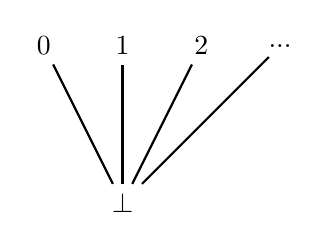
\begin{tikzpicture}
    \node (top) at (0,0) {$\bot$};
    \node (a) at (-1,2) {0};
    \node (b) at (0,2) {1};
    \node (c) at (1,2) {2};
    \node (d) at (2,2) {...};
    \draw [thick] (top) -- (a);
    \draw [thick] (top) -- (b);
    \draw [thick] (top) -- (c);
    \draw [thick] (top) -- (d);
\end{tikzpicture}
\end{center}

\vspace{0.5cm}

Now we must prove that this is a domain:

\vspace{0.5cm}

\begin{lem}
$(\mathbbm{N}, \bot, \sqsubseteq)$ is a domain.
\end{lem} 

\begin{proof}
We prove the three conditions in the domain definition:

In the definition of our relation we have $\{ (\bot , n) \ | \ n \in \mathbb{N} \}$, so $\forall x \in \mathbb{N}. \ \bot \sqsubseteq x$.

Next, we prove $\sqsubseteq$ is a partial order. From the  definition of $\sqsubseteq$, we have $\{(x,x) \ | \ x \in \natb \}$, which is a subset of $\sqsubseteq$, so $\sqsubseteq$ must be reflexive.

We prove antisymmetry by case analysis. When $x = \bot$, the only possible $y$ we can have such that $y \sqsubseteq x$ is $y = \bot$, as  $n \sqsubseteq \bot$ is not defined in the relation for any $n$. Therefore $x = y = \bot$. When $x = n$, the only possible value of $y$ is $n$, so $x = y = n$. Therefore every element of the underlying set satisfies antisymmetry.

We also prove transitivity by case analysis. If $x = \bot$ and $y =n$, then we must have $z = n$ for $(y,z)$ to be in $\sqsubseteq$. Then we need $\bot \sqsubseteq n$ , which we have, as $(\bot, n)$, for any $n \in \mathbb{N}$ is defined in the relation. If $x = \bot = y$, then we have two options for $z$. When $z = n$, we should have $\bot \sqsubseteq n$, which we have, as $(\bot, n)$ for any $n \in \mathbb{N}$ is defined in the relation. When $z = \bot$, we want $ \bot \sqsubseteq \bot$, which is also in the definition of $\sqsubseteq$. If $x = n$, then both $y$ and $z$ must also be equal to $n$ for $x \sqsubseteq y$ and $y \sqsubseteq z$ to be defined. Therefore we should  have $n \sqsubseteq n$. This is in the definition of $\sqsubseteq$.

Finally we prove that all chains must have a least upper bound. We prove this by case analysis on the different chains. For  chains of the form $\bot \sqsubseteq \dots \sqsubseteq \bot$, let $z = \bot$. The last element in the chain will always be $\bot$, so for every $i$ we have $\bot \sqsubseteq \bot$. Therefore $\forall i . x_i \sqsubseteq \bot$.
For the second statement, as every element is $\bot$, $x_i = \bot$ and $y = \bot$, we have $\bot \sqsubseteq \bot$ for $z \sqsubseteq y$. Therefore $\forall y. (\forall i . x_i \sqsubseteq y) \Rightarrow \bot \sqsubseteq y$ holds.

For chains of the form $n \sqsubseteq \dots \sqsubseteq n$, let $z = n$. The last element in the chain will always be $n$, so for every $n$ we have $n \sqsubseteq n$. Therefore $\forall i . x_i \sqsubseteq n$. For the second part, every element is $n$, so $x_i = n$ and $y = n$. Then we have $n \sqsubseteq n$ for $z \sqsubseteq y$. Therefore $\forall y. (\forall i . x_i \sqsubseteq y) \Rightarrow n \sqsubseteq y$ holds.

For chains of the form $\bot \sqsubseteq \dots \sqsubseteq \bot \sqsubseteq n \sqsubseteq \dots \sqsubseteq n$, let $z = n$.  The last element will be $n$. We have both $\bot \sqsubseteq n$ and $n \sqsubseteq n$ in the relation, so for any $x$, we have $x \sqsubseteq n$. Therefore $\forall i . x_i \sqsubseteq n$. For the second part, $(\forall i . x_i \sqsubseteq y)$ is only true when $y = n$, so we only have to consider this case. Then we have $n \sqsubseteq n$ for $z \sqsubseteq y$. Therefore $\forall y. (\forall i . x_i \sqsubseteq y) \Rightarrow n \sqsubseteq y$ holds.
\end{proof}

\subsection{Product of domains}\label{prod}
Given two domains $\mathbb{X} = (X, \bot_X, \sqsubseteq_X)$ and $\mathbb{Y} = (Y, \bot_Y, \leq_Y)$, we have a new domain,  where $X \times Y$ is the underlying set, the bottom element is $(\bot_X, \bot_Y)$ and $(x,y) \sqsubseteq (x',y')$ is defined when $x \sqsubseteq_X x'$ and $y \leq_Y y'$ are defined.

\vspace{0.25cm}

Now we must prove that this is a domain.

\vspace{0.5cm}

\begin{lem}
$(X \times Y, (\bot_X, \bot_Y), \sqsubseteq)$ is a domain
\end{lem}

\begin{proof}
We prove the three conditions in the domain definition:

As $\mathbbm{X}$ is a domain, we know $\forall x \in X. \ \bot_X \sqsubseteq_X x$ and because $\mathbb{Y}$ is a domain, we know $\forall y \in Y. \ \bot_Y \leq_Y y$. Therefore we have $\forall x,y . \ \bot_X \sqsubseteq_X x \wedge \bot_Y \leq_Y y$. This is the same as $\forall (x,y) \in X \times Y. (\bot_X,\bot_Y) \sqsubseteq (x,y)$.

Next, we prove $\sqsubseteq $ is a partial order. For an element $(x,y) \in X \times Y$, we have $x \sqsubseteq_X x$ and $y \leq_Y y$ because $\mathbb{X}$ and $\mathbb{Y}$ are domains, so their orderings are reflexive. This means we have $(x,y) \sqsubseteq (x,y)$, so $\sqsubseteq$ is also reflexive. For elements $(x,y)$ and $(x',y')$ we can assume $(x,y) \sqsubseteq (x',y')$ and $(x',y') \sqsubseteq (x,y)$. Expanding these definitions we have $x \sqsubseteq_X x' \wedge y \leq_Y y' \wedge x' \sqsubseteq_X x \wedge y' \leq_Y y$. If we reorder this we have:

\[x \sqsubseteq_X x' \wedge x' \sqsubseteq_X x \wedge y \leq_Y y' \wedge y' \leq_Y y \]

As the orderings on $\mathbb{X}$ and $\mathbb{Y}$ are antisymmetric, we can rewrite this as $x = x'$ and $y = y'$. Therefore we have $(x,y) = (x',y')$, so $\sqsubseteq$ is antisymmetric. For elements $(x,y), (x',y')$ and $(x'',y'')$ we can assume $(x,y) \sqsubseteq (x',y')$ and $(x',y') \sqsubseteq (x'',y'')$. Expanding these definitions gives us $x \sqsubseteq_X x' \ \wedge \ y \leq_Y y' \wedge \ x' \sqsubseteq_X x'' \wedge y' \leq_Y y''$. If we reorder this we have:


\[x \sqsubseteq_X x' \wedge x' \sqsubseteq_X x'' \wedge y \leq_Y y' \wedge y' \leq_Y y'' \]

As the orderings on $\mathbb{X}$ and $\mathbb{Y}$ are transitive, we can rewrite this as $x \sqsubseteq_X x''$ and $y \leq_Y y''$. Therefore we can now define $(x,y) \sqsubseteq (x'',y'')$, so $\sqsubseteq$ is transitive.

Finally we prove that all chains have a least upper bound. Chains of $\mathbbm{X \times Y}$ will be of the form:

\[(x,y) \sqsubseteq (x', y') \sqsubseteq (x'', y'') \sqsubseteq \dots \]

where $x \sqsubseteq_X x' \sqsubseteq_X x'' \dots$ and $y \leq_Y y' \leq_Y y'' \dots $.

Let $z = \bigsqcup (x, y)_n = (\bigsqcup x_n, \bigsqcup y_n)$. Then as $\mathbb{X}$ and $\mathbb{Y}$ are domains, we have $\forall i. \ x_i \sqsubseteq_X \bigsqcup x_n$ and  $\forall i. \  y_i \leq_Y \bigsqcup y_n$. Therefore, for any $(x,y)$ we have $\forall i. (x_i ,y_i) \sqsubseteq (\bigsqcup x_n , \bigsqcup y_n)$.

%\item{$\forall (x',y'). \ (\forall i . (x_i,y_i) \sqsubseteq (x',y')) \Rightarrow z \sqsubseteq (x',y')$\\
As $\mathbb{X}$ and $\mathbb{Y}$ are domains, we have $\forall x'. \  (\forall i.\  x_i \sqsubseteq_X x') \Rightarrow \bigsqcup x_n \sqsubseteq_X x'$ and $\forall y'. \ (\forall i. \ y_i \leq_Y y') \Rightarrow \bigsqcup y_n \leq_Y y'$.

 Therefore if we assume $\forall (x',y'). (\forall i . (x_i,y_i) \sqsubseteq (x',y'))$, then we know $\bigsqcup x_n \sqsubseteq_X x'$ and $\bigsqcup y_n \leq_Y y'$. This is the definition of $(\bigsqcup x_n , \bigsqcup y_n) \sqsubseteq (x',y')$.

\vspace{0.25cm}

Now we have proved all the conditions, so the product of two domains is also a domain.
\end{proof}

\section{Monotone and Continuous Functions}
There are two different types of functions that we will use when modelling PCF functions:

\vspace{0.25cm}

\begin{defn}
A \textbf{monotone} function, $f$, is a function that preserves the order of a partially ordered set, $X$,  so:

\[ \forall x, y \in X. \ x \sqsubseteq y  \Rightarrow f(x) \sqsubseteq f(y) \]
\end{defn}

Given a chain $x_0 \sqsubseteq x_1 \sqsubseteq \dots$, we can form the chain $f(x_0) \sqsubseteq f(x_1) \sqsubseteq \dots$ using a monotone function.

\vspace{0.25cm}

\begin{defn}
A \textbf{continuous} function $f$ is a function which when applied to the limit of a chain gives the same result as the limit of the chain formed by applying $f$ to every element of another chain. Formally:

\[ f(\bigsqcup x_n) = \bigsqcup (f(x_n))\]
\end{defn}

Therefore continuous functions must also be monotone:

\vspace{0.25cm}

\begin{thm}\label{mono}
Continuous functions are monotone
\end{thm}

\begin{proof}
Given a continuous function $f$, on a partially ordered set $X$, we need to show that $\forall x,y \in X. \ x \sqsubseteq y \Rightarrow f(x) \sqsubseteq f(y)$.
Assume we have a chain $x_n$, where $x_0 = x$ and $x_{n + 1} = y$ for all $n$:

\[x \sqsubseteq y \sqsubseteq y \dots \] .

The limit of this chain will be $y$, so $f(\bigsqcup x_n) = f(y) = \bigsqcup (f (x_n))$.

We also know that because there are only two different elements in the chain, $\bigsqcup (f (x_n)) = f(x) \sqcup f(y) = f(y)$, so therefore $f(x) \sqsubseteq f(y)$.

\end{proof}

\subsection{Domain of Continuous Functions}\label{cont}

We can form a domain of continuous functions between two other domains:

Given two domains $\mathbb{X} = (X, \bot_X, \sqsubseteq_X)$ and $\mathbb{Y} = (Y, \bot_Y, \leq_y)$, we can form the set $\cont(X,Y) =\{ f : X \to Y\}$, of continuous functions between the underlying sets, where:

\begin{itemize}
\item{$\forall x, x' \in X. \ x \sqsubseteq_X x' \Rightarrow f(x) \leq_Y f(x')$ \hspace{1cm} $f$ preserves the ordering of chains in $\mathbbm{X}$}
\item{$x_n \in \chain(X) \Rightarrow f(\bigsqcup x_n) = \bigsqcup f(x_n)$ \hspace{2cm} $f$ is continuous}
\end{itemize} 

where $\chain(X)$ is the set of all possible chains we can form from  $\mathbbm{X}$.

$\bot_{X \to Y}$ is defined as the function $\bot = \lambda x. \bot (x)$, the function that loops on all inputs. The output of this function will always be $\bot$, because it does not terminate. 

The relation $\rel$ is defined as

\[ \rel  \ = \{ (f , g) \ | \ f,g \in \cont(X,Y) \ \wedge \ \forall x \in X. \ f(x) \leq_Y g(x)\} \]

Therefore our domain will be $(\cont(X,Y), \bot_{X \to Y}, \sqsubseteq_C)$. Now we must prove that this is a domain.

\vspace{0.5cm}

\begin{lem}
$(\cont(X,Y), \bot_{X \to Y}, \sqsubseteq_C)$ is a domain.
\end{lem}

\begin{proof}
We must prove the three conditions in the domain definition:

For all $x \in X$ we have $\bot \leq_Y f(x)$. As $\mathbb{Y}$ is a domain we know this holds for every element of $Y$ and as the codomain of $f$ is $Y$, every $f(x)$ is in $Y$. Therefore $\forall f \in \cont(X,Y). \ \bot_{X \to Y} \rel f$.

Next we prove $\rel$ is a partial order. As $\mathbb{Y}$ is a domain, we know that $\leq_Y$ is a partial order. For reflexivity, we need to prove that $\forall f \in \cont(X,Y). \ f \rel f$. We can rewrite this using the definition of $\rel$ to get 
\[\forall f \in \cont(X,Y). \ (\forall x \in X. \ f(x) \leq_Y f(x))\]
 Functions are single valued, so we know $\forall f. \ \forall x. \ f(x) = f(x)$ and as $\leq_Y$ is reflexive we know $\forall f. \forall x \in X. \ f(x) \leq_Y f(x)$. Therefore we have $f \rel f$, for any $f \in \cont(X,Y)$. For antisymmetry, we need to prove that $\forall f,g \in \cont(X,Y). \ ((f \rel g) \ \wedge \ (g \rel f)) \Rightarrow f = g$. Rewriting this using the definition of $\rel$ gives us
 \[\forall f,g \in \cont(X,Y). \ (\forall x \in X. \ ((f(x) \leq_Y g(x)) \ \wedge \ (g(x) \leq_Y f(x))) \Rightarrow f(x) = g(x))\] 
 $\leq_Y$ is antisymmetric, so we have $\forall x \in X. \ f(x) = g(x)$, for any values of $f$ and $g$. Therefore $\rel$ is also antisymmetric. For transitivity, we need to prove that $\forall f,g,h \in \cont(X,Y). \ ((f \rel g) \  \wedge \ (g \rel h)) \Rightarrow f \rel h$. Rewriting this using the definition of $\rel$ gives us 
 \[\forall f,g,h \in \cont(X,Y). \ (\forall x \in X. \ ((f(x) \leq_Y g(x)) \ \wedge \ (g(x) \leq_Y h(x))) \Rightarrow f(x) \rel h(x)) \]
 
As $\leq_Y$ is transitive, we have $\forall x \in X.f(x) \leq_Y h(x)$, for all $f, g$ and $h$. Therefore $\rel$ is also transitive. 

Finally we prove that all chains have a least upper bound. Let $z = \lambda x. \bigsqcup^Y f_n (x)$, where $\bigsqcup^Y f_n (x)$ is the limit of the chain (in $\mathbbm{Y}$) obtained by applying the functions in some chain of elements of $\cont(X,Y)$ to a certain element $x \in X$.

An example of a chain of such functions is:

\[ f_1 \rel f_2 \rel \dots \rel \bigsqcup f_n \]

If we expand this using the definition of $\rel$ we have

\[ \forall x \in X. \ (f_1(x) \leq_y f_2(x) \leq_Y \dots \leq_Y \bigsqcup f_n (x)) \]

This is a set of chains in $\chain(Y)$ where every chain contains the result of each function on a certain $x \in X_\bot$. As $\mathbb{Y}$ is a domain, the least upper bound is defined for any chain using the elements of $Y_\bot$. Therefore we know that the least upper bound $\bigsqcup f_n (x)$ is defined. Now we can see that this is the same as our definition of $z$, which was $\lambda x. \bigsqcup^Y f_n (x)$.

For the second part of the proof, we can rewrite it using the definition of $\rel$ as

\[ \forall x \in X. \ (\forall g. (\forall i . f_i(x) \leq_Y g(x)) \Rightarrow z(x) \leq_Y g(x)) \]


As $\mathbbm{Y}$ is  a domain, $(\forall i . f_i(x) \leq_Y g(x)) \Rightarrow z(x) \leq_Y g(x))$ holds for each of our individual chains for each $x \in X$. Therefore we have $ \forall g. (\forall i . f_i \rel g) \Rightarrow z \rel g$
\end{proof}


\section{Fixpoint Theorem}\label{fixpoint}

Now we have a domain of continuous functions, we can use it to state and prove the fixpoint theorem. The following theorem is an important result in recursion theory, that we will use to model recursion in PCF. The chain given in the theorem is the chain obtained by repeatedly iterating a recursive function on its previous result, starting with $\bot$. If an input of the function is computed using $f^n(\bot)$ and it needs more than $n$ iterations then it will not terminate. As the chain can be infinitely long, it can model infinite (general) recursion.

\vspace{0.5cm}


\begin{thm}
Every continuous function $f : X \to X$ has a least fixpoint, which is the limit of the chain $\bot \sqsubseteq f(\bot) \sqsubseteq f^2(\bot) \sqsubseteq \dots$
\end{thm}

\begin{proof}
 Define the fixpoint function $fix(f) \equiv \bigsqcup f^n (\bot)$. This is the limit of the chain in the theorem. We know this limit exists because $f$ is continuous, so $(X, \bot, \sqsubseteq)$ must form a domain (see Section \ref{cont}), and by the definition of domain, all chains of $\mathbbm{X}$ have a limit. 

%First we must prove that this limit exists, so $\forall i \in \mathbb{N} . \ f^i(\bot) \sqsubseteq f^n(\bot)$. We prove this by induction. If $i = 0$, then the only element of the chain is $f^0(\bot) = \bot$. $\bot$ is the least element of the chain, so we have $\bot  \sqsubseteq f^n(\bot)$. 

%The inductive hypothesis is $\sqcup f^i(\bot)$ exists. Applying $f$ to this gives us $f(\sqcup f^i(\bot))$. $f$ is continuous, so this is equal to $\sqcup f(f^i(\bot)) = \sqcup f^{i+1}(\bot) $

\paragraph{$\bigsqcup f^n (\bot)$ is a fixpoint}
For the limit to be a fixpoint we must have  $f( \bigsqcup f^n (\bot)) =  \bigsqcup f^n (\bot)$.  As $f$ is continuous, we have $f( \bigsqcup f^n (\bot)) = \bigsqcup f(f^n(\bot)) = \bigsqcup f^{n+1}(\bot)$. The chain formed by $f^{n+1}$ is $f(\bot)  \sqsubseteq f^2(\bot) \sqsubseteq \dots$. This is the same as our original chain, but without $\bot$ at the start. Because $\mathbbm{X}$ is a domain, we know that $\forall x \in X. \ \bot \sqsubseteq x$. Therefore $\bot$ has no effect on the limit because every element is higher than it, so removing $\bot$ will not change the limit. This means that $\bigsqcup f^{n+1} (\bot) = \bigsqcup f^n(\bot)$.

\paragraph{$\bigsqcup f^n (\bot)$ is the least fixpoint}
Let $x$ be an element of our chain such that $fix(x) = x$. Then for $\bigsqcup f^n (\bot)$ to be the least fixpoint, we must have $\bigsqcup f^n (\bot) \sqsubseteq x$ (i.e.\ so $x$ is an upper bound that is higher than $\bigsqcup f^n (\bot)$). First we prove $x$ is an upper bound, so  we must show $\forall n. \ f^n(\bot) \sqsubseteq x$. We prove by this by induction on $n$:

if $n = 0$, then $f^0(\bot) \sqsubseteq x$, This is the same as $\bot \sqsubseteq x$, which is true because $\bot$ is the least element of the chain.

Our inductive hypothesis is $f^n(\bot) \sqsubseteq x$. As $f$ is continuous, $f$ is monotone, so $f(f^n(\bot)) \sqsubseteq f(x) = f^{n+1}(\bot) \sqsubseteq x$. Therefore we know that for any element $f^n(\bot)$ in the chain, $f^n(\bot) \sqsubseteq x$. 

As $\bigsqcup f^n (\bot)$ is a least upper bound, we know that  $\forall x \in X. \  \forall n. \ (f^n(\bot) \sqsubseteq x) \Rightarrow \bigsqcup f^n (\bot) \sqsubseteq x$. We have just proved the left hand side of this, so we now have $\bigsqcup f^n (\bot) \sqsubseteq x$.

\vspace{0.5cm}

Now we have proved that $\bigsqcup f^n (\bot)$ is the least fixpoint of $f$.
\end{proof}

Now that we have proved the above theorem, we know enough Domain Theory to model recursive PCF programs of any type.